% !TEX program = xelatex
% =====================================================================
%  CUADebug -- EMNLP 2026 poster  |  A0 PORTRAIT, 841 x 1189 mm
%  15 mm margins -> text block 811 x 1159 mm.
%  One reading path, top to bottom:
%    header band  : title, authors, affiliations | EMNLP logo, school logos
%    key results  : 11.1 -> 19.4% | 61.77 -> 68.14% | QR codes (Paper, Project, Code, Data)
%    row 1        : 1 Motivation | 2 CUAErrorBench | 3 Error Taxonomy
%    row 2        : 4 A Real Failure  (paper teaser, full width)
%    row 3        : 5 CUADebugger     (paper pipeline figure, full width)
%    row 4        : 6 Results         (RCA chart | re-execution table | recovered failures)
%  The key-results band and Results share one 3-column grid (257 mm columns, 20 mm gutters).
%  Open layout: no frames; every section starts with a numbered badge, its title and a rule.
%  Row gaps stretch equally (about 20 mm), so the last row always ends on the bottom margin.
%  Type: title 90 pt, key numbers 80 pt, section titles 54 pt, panel titles and key-result
%  labels 36 pt, body 33 pt, nothing outside the paper figures below 24 pt (superscripts aside).
%  Compile with XeLaTeX (fontspec + OpenType fonts; Overleaf: Menu -> Compiler -> XeLaTeX).
% =====================================================================
\RequirePackage{fix-cm}% scalable CM math fonts (used by \textsuperscript)
\documentclass{article}
\usepackage[paperwidth=841mm,paperheight=1189mm,margin=15mm]{geometry}
\usepackage{fontspec}
\usepackage{xcolor}
\usepackage{colortbl}
\usepackage{graphicx}
\usepackage{tikz}
\usetikzlibrary{arrows.meta}
\usepackage{pgfplots}
\pgfplotsset{compat=1.18}
\usepackage{tcolorbox}
\tcbuselibrary{skins}
\usepackage{qrcode}
\usepackage{array,booktabs,tabularx}
\usepackage{enumitem}
\usepackage{microtype}
\usepackage{hyperref}
\hypersetup{hidelinks, pdfpagemode=UseNone, pdfstartview=Fit,
  pdftitle={CUADebug: Diagnosing and Repairing Computer-Use Agent Failures (EMNLP 2026 poster)}}

% QR codes: qrcode.sty sets every dark module as its own \rule, and screen renderers that
% anti-alias leave hairline seams between neighbouring rules (a faint grid on screen, which
% also makes a code shown on a screen harder to scan).  Its two printing routines are
% replaced by one that draws a code as a single filled path, one rectangle per run of dark
% modules in a row, with the same module size, module positions and box size.
\makeatletter
\newcount\qr@pathrow \newcount\qr@pathcol \newcount\qr@runstart \newcount\qr@pathn
\newdimen\qr@pathx \newdimen\qr@pathy \newdimen\qr@pathw \newdimen\qr@pathoff
\let\qr@printmatrix@rules\qr@printmatrix
\def\qr@printmatrix#1{% first use of a code: print the bits it has just saved
  \ifqr@draft@mode\qr@printmatrix@rules{#1}%
  \else\expandafter\qr@printsavedbinarymatrix\expandafter{\qr@binarymatrix@result}\fi}
\def\qr@printsavedbinarymatrix#1{% #1 expands to the modules, row by row from the top (1 = dark)
  \edef\qr@pathbits{#1}%
  \setlength{\qr@modulesize}{\qr@desiredheight}%
  \divide\qr@modulesize by \qr@size\relax
  \setlength{\qr@minipagewidth}{\qr@modulesize}%
  \multiply\qr@minipagewidth by \qr@size\relax
  \qr@pathoff=\z@
  \ifqr@tight\else
    \qr@pathoff=4\qr@modulesize
    \advance\qr@minipagewidth by 8\qr@modulesize
  \fi
  \colorlet{qr@pathcolor}{.}% the text colour, which the rules took
  \begin{pgfpicture}% (inside the tile's node: drop its transformation and rounded corners)
    \pgftransformreset
    \pgfsetcornersarced{\pgfpointorigin}%
    \pgfsetfillcolor{qr@pathcolor}%
    \pgfpathrectangle{\pgfpointorigin}{\pgfqpoint{\qr@minipagewidth}{\qr@minipagewidth}}%
    \pgfusepath{use as bounding box}%
    \qr@pathrow=\z@ \qr@pathcol=\z@ \qr@runstart=\m@ne
    \expandafter\qr@pathscan\qr@pathbits\relax
    \pgfusepath{fill}%
  \end{pgfpicture}}
\def\qr@pathscan#1{%
  \ifx\relax#1\else
    \if1#1\ifnum\qr@runstart<\z@ \qr@runstart=\qr@pathcol \fi
    \else\ifnum\qr@runstart<\z@ \else\qr@pathrun\fi
    \fi
    \advance\qr@pathcol\@ne
    \ifnum\qr@pathcol=\qr@size\relax
      \ifnum\qr@runstart<\z@ \else\qr@pathrun\fi
      \qr@pathcol=\z@ \advance\qr@pathrow\@ne
    \fi
    \expandafter\qr@pathscan
  \fi}
\def\qr@pathrun{% dark run: columns \qr@runstart .. \qr@pathcol-1 of row \qr@pathrow
  \qr@pathx=\qr@runstart\qr@modulesize \advance\qr@pathx\qr@pathoff
  \qr@pathn=\qr@pathcol \advance\qr@pathn-\qr@runstart
  \qr@pathw=\qr@pathn\qr@modulesize
  \qr@pathn=\qr@size\relax \advance\qr@pathn-\qr@pathrow \advance\qr@pathn\m@ne
  \qr@pathy=\qr@pathn\qr@modulesize \advance\qr@pathy\qr@pathoff
  \pgfpathrectangle{\pgfqpoint{\qr@pathx}{\qr@pathy}}{\pgfqpoint{\qr@pathw}{\qr@modulesize}}%
  \qr@runstart=\m@ne}
\makeatother

% ---------------------------------------------------------------------
%  Fonts: TeX Gyre Heros (Helvetica)
% ---------------------------------------------------------------------
\setmainfont{texgyreheros}[Extension=.otf, UprightFont=*-regular, BoldFont=*-bold,
  ItalicFont=*-italic, BoldItalicFont=*-bolditalic]

\makeatletter
\renewcommand\tiny        {\@setfontsize\tiny        {24pt}{28pt}}
\renewcommand\scriptsize  {\@setfontsize\scriptsize  {24pt}{28pt}}
\renewcommand\footnotesize{\@setfontsize\footnotesize{25pt}{30pt}}
\renewcommand\small       {\@setfontsize\small       {28pt}{34pt}}
\renewcommand\normalsize  {\@setfontsize\normalsize  {33pt}{41pt}}
\renewcommand\large       {\@setfontsize\large       {36pt}{43pt}}
\renewcommand\Large       {\@setfontsize\Large       {44pt}{52pt}}
\renewcommand\LARGE       {\@setfontsize\LARGE       {54pt}{62pt}}
\renewcommand\huge        {\@setfontsize\huge        {70pt}{78pt}}
\renewcommand\Huge        {\@setfontsize\Huge        {90pt}{96pt}}
\makeatother
% superscripts in the author block (\textsuperscript takes the math script size):
% 24 pt on the 33 pt author line, 20 pt on the 27 pt affiliation line
\DeclareMathSizes{33}{33}{24}{17}
\DeclareMathSizes{27}{27}{20}{14}

% ---------------------------------------------------------------------
%  Colours (blue/teal/red and family colours as in the paper figures)
% ---------------------------------------------------------------------
\definecolor{navy}{HTML}{0F2742}       % header band, titles
\definecolor{headsub}{HTML}{C3D3E8}    % secondary text on the band
\definecolor{titleacc}{HTML}{9CC4F2}   % "CUADebug:" on the band
\definecolor{ink}{HTML}{1C1C1C}
\definecolor{muted}{HTML}{5D6670}
\definecolor{rulec}{HTML}{CBD5E1}
\definecolor{tint}{HTML}{EAF1FA}       % key-results band
\definecolor{bandline}{HTML}{BCCDE3}   % rules inside the band
\definecolor{ours}{HTML}{1F5FAD}       % our method
\definecolor{basegray}{HTML}{A7AFBA}
\definecolor{before}{HTML}{6E7887}     % "before" value in the key results (3.9:1 on the tint)
\definecolor{rootred}{HTML}{D93632}    % "root cause" red of the teaser figure
\definecolor{failorange}{HTML}{C98500} % "observed failure" orange of the teaser figure
\definecolor{famP}{HTML}{4E79A7}
\definecolor{famG}{HTML}{F28E2B}
\definecolor{famR}{HTML}{59A14F}
\definecolor{famS}{HTML}{B07AA1}
\definecolor{famO}{HTML}{9C755F}
% colours of the paper figures, for the crop repairs below.  xdvipdfmx writes colours with
% 3 decimals; these values quantise to the same 8-bit colour as the figures' own
% (.0706 .2471 .4745 / .0314 .4863 .5137 / .7804 .2078 .1725 / .7882 .5216 0 /
% .1373 .4196 .2078 and the 7.8 % drop shadow) whether a renderer rounds or truncates.
\definecolor{fgRealcase}{rgb}{0.071,0.248,0.474}
\definecolor{fgTeal}{rgb}{0.032,0.487,0.513}
\definecolor{fgRed}{rgb}{0.781,0.207,0.172}
\definecolor{fgOrange}{rgb}{0.788,0.522,0}
\definecolor{fgGreen}{rgb}{0.138,0.419,0.207}
\definecolor{fgShadow}{rgb}{0.930,0.934,0.942}

\setlength{\parindent}{0pt}
\setlength{\parskip}{0pt}
\setlength{\maxdepth}{0pt}% the last row may not hang into the bottom margin
\hyphenpenalty=10000 \exhyphenpenalty=10000
\setlist{nosep}

% ---------------------------------------------------------------------
%  Grid
% ---------------------------------------------------------------------
\newlength{\gutter}\setlength{\gutter}{20mm}    % between columns
% between rows: at least 19.25 mm plus an equal share of the spare height (about 20 mm here;
% the margin under 20 mm leaves ~4 mm of tolerance for other TeX installations)
\newlength{\rowgap}\setlength{\rowgap}{19.25mm}
\newlength{\headgap}\setlength{\headgap}{6.3mm} % section header line (fixed 4.6 mm depth) -> content
\newcommand{\rowsep}{\par\nointerlineskip\vspace{\dimexpr\rowgap\relax plus 1fill}}
% 3-column grid for the key-results band and Results: 257 | 257 | 257 mm
\newlength{\thirdw}\setlength{\thirdw}{\dimexpr(\textwidth-2\gutter)/3\relax}
% row 1: 1 Motivation | 2 CUAErrorBench | 3 Error Taxonomy
\newlength{\colA}\setlength{\colA}{176mm}
\newlength{\colC}\setlength{\colC}{215mm}
\newlength{\colB}\setlength{\colB}{\dimexpr\textwidth-\colA-\colC-2\gutter\relax}
\newlength{\rowAh}\setlength{\rowAh}{145.5mm}    % content height of row 1
\newlength{\donutD}\setlength{\donutD}{146.2mm}  % donut diameter
\newlength{\plotH}\setlength{\plotH}{109mm}    % Results: plot areas of the two charts
% Results: blank space between a chart's left edge and the start of its widest y tick label
% (measured; mostly the label nodes' padding); each chart is moved left by it and widened by
% the same amount, so the labels start flush with the panel titles and the right ends stay
\newlength{\ylabshift}\setlength{\ylabshift}{3.86mm}

% ---------------------------------------------------------------------
%  Section headers
% ---------------------------------------------------------------------
% numbered badge: a 23.5 mm disc (larger than the step and panel discs inside the figures,
% so the six section numbers read as the top level); it takes a line box only 19 mm high
% (the disc overhangs it by 2.25 mm above and below), so the header lines keep their height
\newcommand{\badge}[1]{\tikz[baseline={([yshift=-6.6mm]b.center)}]{%
  \node[circle, fill=navy, text=white, font=\fontsize{48pt}{48pt}\selectfont\bfseries,
        minimum size=23.5mm, inner sep=0pt, overlay](b){#1};
  \path (b.center) ++(-11.75mm,-9.5mm) rectangle ++(23.5mm,19mm);}}
% title with its descenders ignored; \secstrut gives every header line the same depth,
% so content starts at the same distance under every header
\newcommand{\sectitle}[1]{\raisebox{0pt}[\height][0pt]{\LARGE\bfseries\color{navy}#1}}
\newcommand{\secstrut}{\rule[-4.6mm]{0pt}{4.6mm}}
% column / full-width section: badge, title, rule to the column edge
\newcommand{\sechead}[2]{%
  \noindent\secstrut\badge{#1}\hspace{6mm}\sectitle{#2}%
  \hspace{9mm}{\color{rulec}\leaders\hrule height 7.1mm depth -6.1mm\hfill}%
  \par\nointerlineskip\vspace{\headgap}}
% full-width figure section: badge, title, divider, lead sentence(s) (first line on the
% title's baseline; a second sentence starts its own line)
\newsavebox{\ledehead}
\newcommand{\secheadlede}[3]{%
  \sbox{\ledehead}{\badge{#1}\hspace{6mm}\sectitle{#2}\hspace{9mm}%
    {\color{rulec}\vrule width 1.2mm height 14mm depth 2.5mm}\hspace{9mm}}%
  \noindent\secstrut\usebox{\ledehead}%
  \parbox[t]{\dimexpr\linewidth-\wd\ledehead\relax}{\normalsize\raggedright#3\secstrut}%
  \par\nointerlineskip\vspace{\headgap}}

% ---------------------------------------------------------------------
%  Header pieces
% ---------------------------------------------------------------------
\newlength{\hright}\setlength{\hright}{180mm}   % logo block at the right of the title
% school logos (white versions), identical height, spread over the logo block
\newcommand{\unirow}[1]{% height
  \makebox[\hright][s]{%
  
\includegraphics[height=#1, trim=0.66bp 0.72bp 0.78bp 0.78bp, clip]{logos/illinois_white.pdf}\hfill
  
\includegraphics[height=#1]{logos/stanford_white.pdf}\hfill
  
\includegraphics[height=#1]{logos/yale_white.pdf}}}
% QR code: 38 mm code on a white tile with a quiet zone of more than 4 modules, label below;
% the tile links to the URL (\XeTeXLinkBox: xdvipdfmx sizes a link by the glyphs inside it,
% and a code has none; with other engines it is a plain box)
\newlength{\qrsize}\setlength{\qrsize}{38mm}
\newlength{\qrpad}\setlength{\qrpad}{5.5mm}
\newcommand{\hqr}[2]{% label, url
  \begin{minipage}[t]{\dimexpr\qrsize+2\qrpad\relax}\centering
    \href{#2}{\XeTeXLinkBox{\tikz\node[fill=white, rounded corners=1.5mm, inner sep=\qrpad]
      {\qrcode[nolink,height=\qrsize,level=M]{#2}};}}\par
    \vspace{1.3mm}{\fontsize{24pt}{26pt}\selectfont\color{ink}#1\par}
  \end{minipage}}
% key result: before value (grey) -> after value (blue), label
\newcommand{\kpi}[3]{%
  {\fontsize{58pt}{60pt}\selectfont\bfseries\color{before}#1\hspace{0.16em}→\hspace{0.16em}}%
  {\fontsize{80pt}{84pt}\selectfont\bfseries\color{ours}#2\par}%
  \vspace{4.5mm}{\large\color{ink}#3\rule[-0.25em]{0pt}{0pt}\par}}% fixed depth: both blocks centre alike

% ---------------------------------------------------------------------
%  Paper figures with crop repairs (coordinates in figure bp, y from the top)
%  Each figure is scaled by an explicit factor \fs = width / crop width, and the overlay
%  uses the same factor (graphicx's width= division is only accurate to about 2e-4,
%  which would shift the overlay by up to 0.2 pt).
% ---------------------------------------------------------------------
% Teaser (Fig. 1, 1200 x 678 bp): task header + "A Failure trajectory" row.
% Crop x 13.4..1186.5, y 37.5..340.45 (frames sit on the crop edges; the right edge is the
% outer edge of panel 5's frame, so no sliver of its drop shadow shows).  Two descenders of
% the cut figure title lie on the task box's top border: the straight top edge (x 21..1179)
% is first covered with white (reaching 1 bp above the crop, onto blank page, so no
% anti-aliased trace of the descenders survives on the crop edge) and then redrawn in its
% own colour at the original 1.5 bp.  The frames of parts B/C start at y = 340.5, just under
% the crop; white masks over the gaps between the trajectory panels (beside their drop
% shadows) make sure no hairline of them can show.  At panel 5's bottom-right corner, the
% last one on the crop's right edge, the crop leaves a wedge of the panel's drop shadow
% outside the rounded frame: it is covered too, and the corner is redrawn with the frame's
% own path at 1.5 bp, overlapping the frame by 1 bp at both ends.  The task box's top-right
% corner, the other corner on the crop's right edge, gets the same repair.
% the task box's top-right frame corner, from (1179,38.25) to (1185.75,45)
\newcommand{\ttaskcorner}{%
  .. controls (1179.4432,38.2500) and (1179.8821,38.2932) .. (1180.3168,38.3797)
  .. controls (1180.7514,38.4662) and (1181.1734,38.5942) .. (1181.5829,38.7638)
  .. controls (1181.9924,38.9334) and (1182.3814,39.1413) .. (1182.7499,39.3876)
  .. controls (1183.1184,39.6338) and (1183.4594,39.9136) .. (1183.7729,40.2270)
  .. controls (1184.0863,40.5404) and (1184.3660,40.8814) .. (1184.6122,41.2499)
  .. controls (1184.8584,41.6184) and (1185.0663,42.0074) .. (1185.2360,42.4169)
  .. controls (1185.4056,42.8264) and (1185.5336,43.2484) .. (1185.6201,43.6831)
  .. controls (1185.7066,44.1178) and (1185.7499,44.5568) .. (1185.7500,45.0000)}
% panel 5's bottom-right frame corner, from (1185.75,331.5) to (1177.5,339.75)
\newcommand{\tfivecorner}{%
  .. controls (1185.7499,332.0417) and (1185.6970,332.5782) .. (1185.5913,333.1094)
  .. controls (1185.4856,333.6407) and (1185.3291,334.1566) .. (1185.1218,334.6570)
  .. controls (1184.9146,335.1576) and (1184.6604,335.6330) .. (1184.3595,336.0834)
  .. controls (1184.0586,336.5338) and (1183.7166,336.9506) .. (1183.3335,337.3336)
  .. controls (1182.9504,337.7166) and (1182.5337,338.0586) .. (1182.0833,338.3596)
  .. controls (1181.6328,338.6605) and (1181.1575,338.9146) .. (1180.6570,339.1220)
  .. controls (1180.1565,339.3293) and (1179.6406,339.4857) .. (1179.1094,339.5915)
  .. controls (1178.5780,339.6971) and (1178.0415,339.7500) .. (1177.5000,339.7500)}
\newcommand{\teaserfig}[1]{%
  \pgfmathsetmacro{\fs}{#1/(1173.1bp)}%
  \begin{tikzpicture}[inner sep=0pt, outer sep=0pt]
    \node[anchor=north west] (img) at (0,0)
      {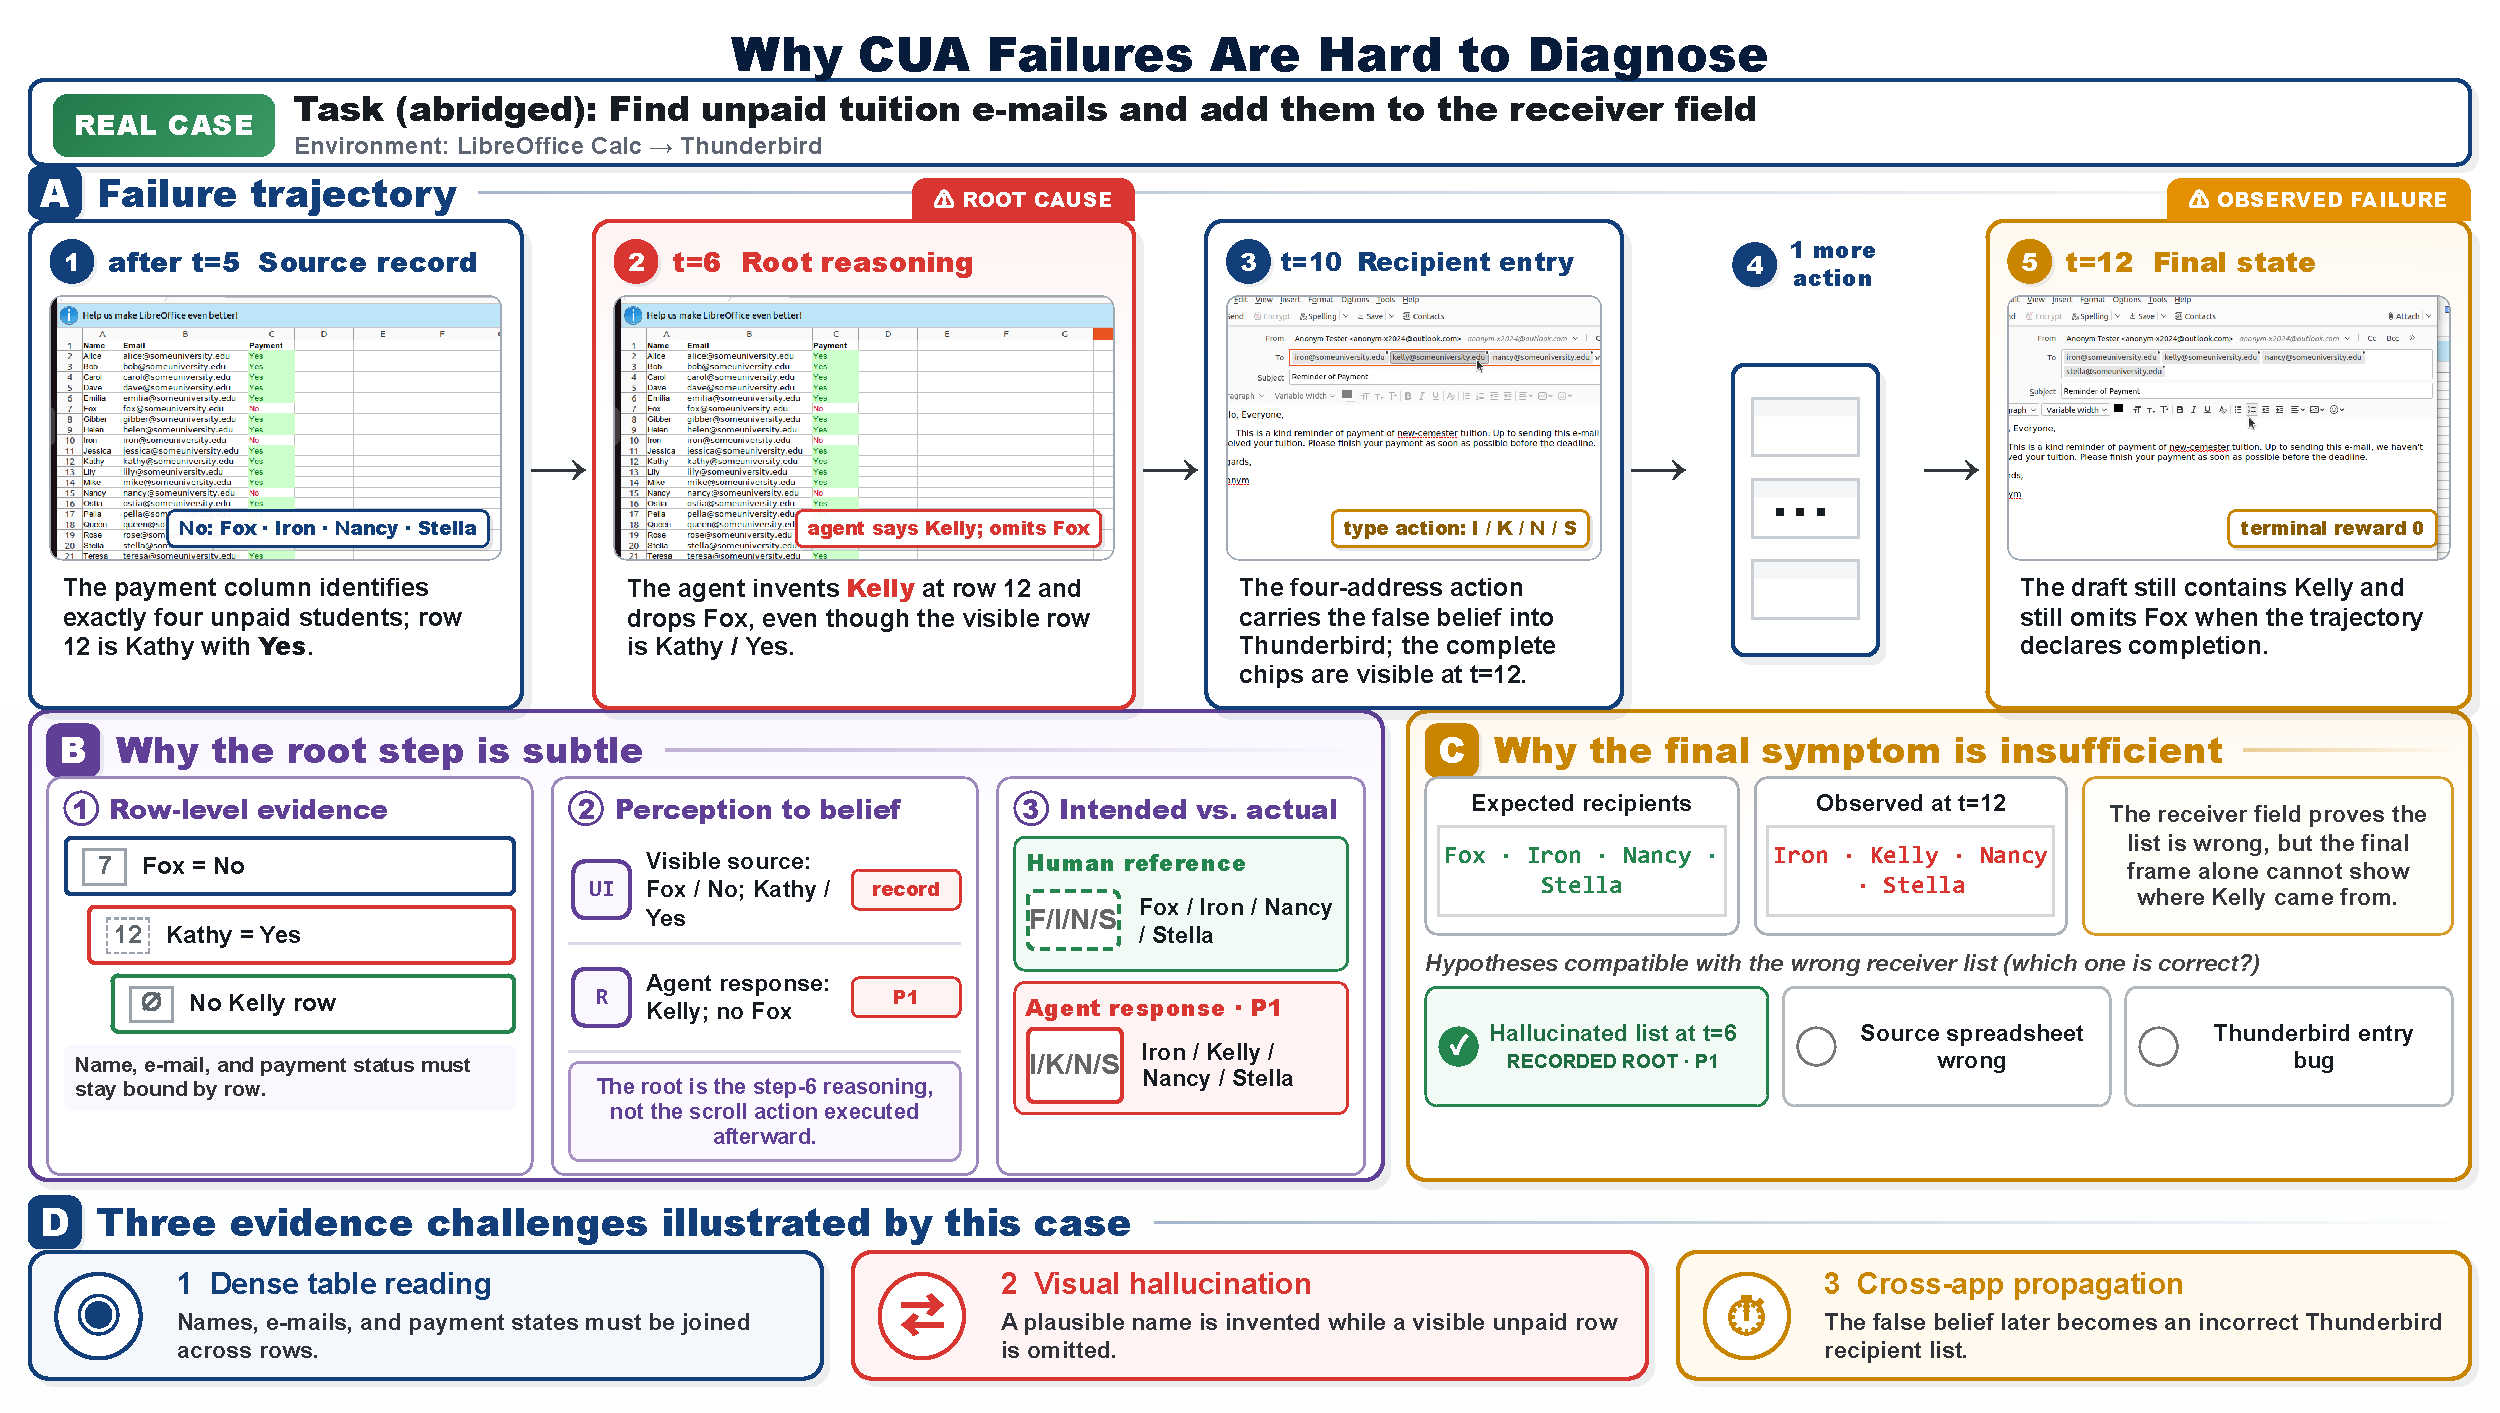
\includegraphics[scale=\fs, trim=13.4bp 337.55bp 13.5bp 37.5bp, clip]{figures/teaser_figure.pdf}};
    \begin{scope}[x=\fs bp, y=-\fs bp, shift={(-13.4,-37.5)}]
      \fill[white] (21.5,36.5) rectangle (1178.5,39.0);
      \draw[fgRealcase, line width=1.5*\fs bp] (20.5,38.25) -- (1179.5,38.25);
      \fill[white] (255.25,339.9) rectangle (284.0,341.5);
      \fill[white] (549.25,339.9) rectangle (578.0,341.5);
      \fill[white] (783.25,339.9) rectangle (953.0,341.5);
      % panel 5's corner (the fill reaches onto blank page; overlay: no change to the bounding box)
      \fill[white, overlay] (1185.75,328.5) -- (1185.75,331.5) \tfivecorner -- (1174.5,339.75)
        -- (1174.5,341.5) -- (1187.5,341.5) -- (1187.5,328.5) -- cycle;
      \begin{scope}
        \clip (1170,320) rectangle (1186.5,340.45);
        \draw[fgOrange, line width=1.5*\fs bp] (1185.75,327.5) -- (1185.75,331.5) \tfivecorner
          -- (1173.5,339.75);
      \end{scope}
      % the task box's top-right corner (its shadow wedge spans y 41.4..45)
      \fill[white, overlay] (1177.5,38.25) -- (1179,38.25) \ttaskcorner -- (1185.75,48.5)
        -- (1187.5,48.5) -- (1187.5,36.5) -- (1177.5,36.5) -- cycle;
      \begin{scope}
        \clip (1170,37.5) rectangle (1186.5,60);
        \draw[fgRealcase, line width=1.5*\fs bp] (1176.5,38.25) -- (1179,38.25) \ttaskcorner
          -- (1185.75,49.5);
      \end{scope}
    \end{scope}
  \end{tikzpicture}}
% Pipeline (Fig. 2, 1200 x 513.12 bp): the four panels only.  Crop x 16.4..1153.5,
% y 58.4..414.75 (right and bottom: the outer edges of the frames, so no sliver of their drop
% shadows shows).  The dropped episodic-memory strip leaves its connector arrow on panel 2's
% OUTPUT bar (masked in the bar's teal and, below the bar, in white).  The strip's title box
% (x 354.24..845.49, from y 413.25 down) hid the bottom of panels 2 and 3 and part of panel
% 2's drop shadow: these are restored with the figure's own paths, and the hidden parts of
% the two bottom edges are redrawn with the figure's own Bezier path at 0.75 bp.
% The figure's background carries a faint tint (a gradient, strongest at the top) in the
% gaps between panels 1 and 2 and between panels 3 and 4, cut off hard by the crop line: it
% is covered down to the connector arrows, so all three gaps are as white as the 2-3 gap.
% Panel 4's top-right and bottom-right corners are repaired like panel 5's in the teaser.
% figures/main_figure.pdf itself carries four typesetting edits, appended as an incremental
% revision (the exported file is its unchanged first part; same words, fonts, sizes and
% colours):
% - the two lines of panel 4's 'Matched continual' box sit 4.75 and 5.25 bp higher, inside the
%   box (the export let 'restart t=51' run over the box's bottom border);
% - panel 2's 'Root:' box breaks before 'omits' instead of leaving 'Fox.' alone on its last line;
% - all four panel titles (disc, its shadow, digit, both lines) sit 2.5 bp higher, so the
%   descenders of panel 1's 'package' no longer run under the TASK box;
% - in panel 4 the Takeaway box is 3 bp higher and 2 bp shorter (its text centred in it) and
%   the OUTPUT bar 1.5 bp higher, level with the other panels' bars, so box and bar no
%   longer touch.
% panel 4's top-right frame corner, from (1143.75,58.875) to (1153.125,68.25)
\newcommand{\pfourtopcorner}{%
  .. controls (1144.3655,58.8750) and (1144.9750,58.9350) .. (1145.5787,59.0551)
  .. controls (1146.1825,59.1752) and (1146.7688,59.3530) .. (1147.3374,59.5886)
  .. controls (1147.9062,59.8242) and (1148.4464,60.1130) .. (1148.9583,60.4550)
  .. controls (1149.4702,60.7969) and (1149.9437,61.1856) .. (1150.3790,61.6209)
  .. controls (1150.8143,62.0561) and (1151.2030,62.5297) .. (1151.5449,63.0415)
  .. controls (1151.8869,63.5533) and (1152.1757,64.0936) .. (1152.4113,64.6623)
  .. controls (1152.6469,65.2310) and (1152.8247,65.8173) .. (1152.9447,66.4210)
  .. controls (1153.0648,67.0248) and (1153.1249,67.6344) .. (1153.1250,68.2500)}
% panel 4's bottom-right frame corner, from (1153.125,405) to (1143.75,414.375)
\newcommand{\pfourcorner}{%
  .. controls (1153.1249,405.6155) and (1153.0648,406.2252) .. (1152.9447,406.8289)
  .. controls (1152.8247,407.4327) and (1152.6470,408.0190) .. (1152.4114,408.5876)
  .. controls (1152.1758,409.1564) and (1151.8870,409.6967) .. (1151.5450,410.2085)
  .. controls (1151.2030,410.7203) and (1150.8145,411.1938) .. (1150.3790,411.6291)
  .. controls (1149.9437,412.0644) and (1149.4701,412.4530) .. (1148.9583,412.7950)
  .. controls (1148.4465,413.1370) and (1147.9062,413.4257) .. (1147.3375,413.6613)
  .. controls (1146.7688,413.8969) and (1146.1826,414.0748) .. (1145.5787,414.1948)
  .. controls (1144.9751,414.3149) and (1144.3655,414.3750) .. (1143.7500,414.3750)}
\newcommand{\mainfig}[1]{%
  \pgfmathsetmacro{\fs}{#1/(1137.1bp)}%
  \begin{tikzpicture}[inner sep=0pt, outer sep=0pt]
    \node[anchor=north west] (img) at (0,0)
      {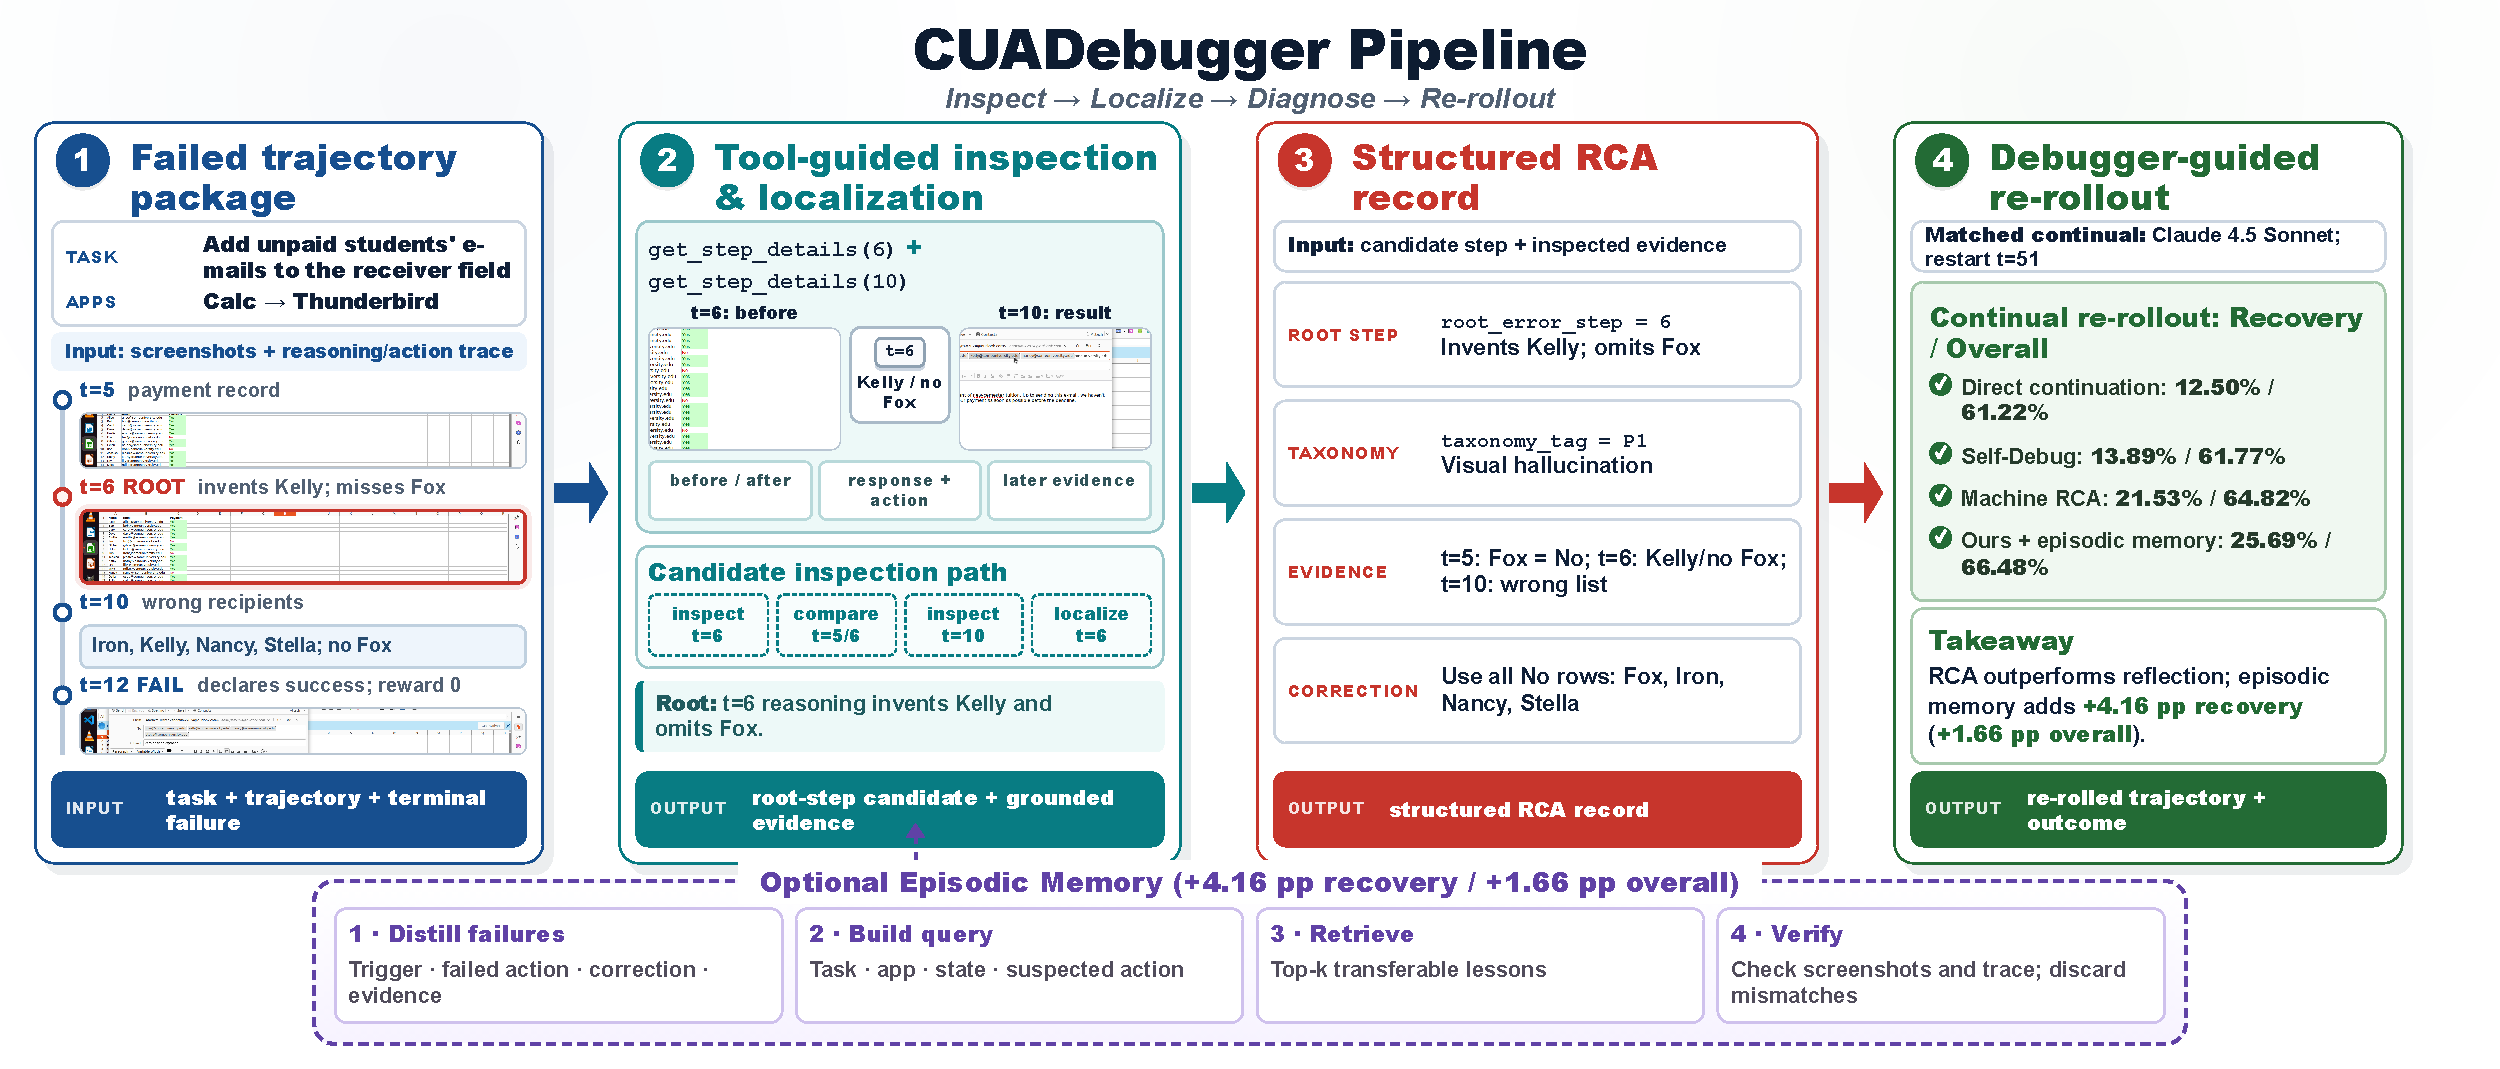
\includegraphics[scale=\fs, trim=16.4bp 98.37bp 46.5bp 58.4bp, clip]{figures/main_figure.pdf}};
    % white covers that reach past the crop onto blank page (overlay: no change to the bounding box)
    \begin{scope}[x=\fs bp, y=-\fs bp, shift={(-16.4,-58.4)}, overlay]
      % gaps 1-2 and 3-4, given by the outer edges of the frames beside them: everything
      % outside the left frame, its drop shadow (4.5 bp further right, from y 63.75) and the
      % right frame (all with 9.75 bp corners), down to just above the arrow.  Each shape is
      % kept 0.15 bp larger, so the fill stays off the anti-aliased edges of the figure's own
      % strokes and shadows; the clip box is larger than the filled box, so no edge of the fill
      % meets an edge of the clip inside a panel (coinciding edges would leave a hairline)
      \foreach \l/\r in {261.0/297.0, 873.0/909.0}{
        \begin{scope}
          \pgfseteorule % each clip: a box around the gap minus one shape
          \clip (\l-20,50) rectangle (\r+20,240)
            [rounded corners=9.9*\fs bp] (\l-60,58.35) rectangle (\l+0.15,300);
          \clip (\l-20,50) rectangle (\r+20,240)
            [rounded corners=9.9*\fs bp] (\l-60,63.6) rectangle (\l+4.65,300);
          \clip (\l-20,50) rectangle (\r+20,240)
            [rounded corners=9.9*\fs bp] (\r-0.15,58.35) rectangle (\r+60,300);
          \fill[white] (\l-12,57) rectangle (\r+12,221.5);
        \end{scope}}
      % panel 4's corners: the shadow wedges outside the frame's rounded corners
      \fill[white] (1153.125,402.5) -- (1153.125,405) \pfourcorner -- (1141.5,414.375)
        -- (1141.5,416) -- (1155,416) -- (1155,402.5) -- cycle;
      \fill[white] (1141.5,58.875) -- (1143.75,58.875) \pfourtopcorner -- (1153.125,71)
        -- (1155,71) -- (1155,56.5) -- (1141.5,56.5) -- cycle;
    \end{scope}
    \begin{scope}
      \clip (img.south west) rectangle (img.north east);
      \begin{scope}[x=\fs bp, y=-\fs bp, shift={(-16.4,-58.4)}]
        % panel 4's corners, redrawn at 0.75 bp, overlapping the frame by 1 bp at both ends
        \draw[fgGreen, line width=0.75*\fs bp] (1153.125,401.5) -- (1153.125,405) \pfourcorner
          -- (1140.5,414.375);
        \draw[fgGreen, line width=0.75*\fs bp] (1140.5,58.875) -- (1143.75,58.875) \pfourtopcorner
          -- (1153.125,72);
        % connector arrow: head and first dash on the bar, second dash under it
        \fill[fgTeal] (434.5,394.8) rectangle (444.5,405.5);
        \fill[white] (437.4,408.6) rectangle (441.6,413.6);
        % area under the strip's title box
        \begin{scope}
          \clip (354.24,413.25) rectangle (845.49,420);
          % drop shadows of panels 2 and 3
          \fill[fgShadow] (354,405) -- (571.5,405) -- (571.5,410.25)
            .. controls (571.5,410.89) and (571.438,411.524) .. (571.313,412.152)
            .. controls (571.188,412.78) and (571.003,413.39) .. (570.758,413.981)
            .. controls (570.513,414.573) and (570.212,415.134) .. (569.857,415.667)
            .. controls (569.501,416.199) and (569.097,416.692) .. (568.644,417.144)
            .. controls (568.192,417.597) and (567.699,418.001) .. (567.167,418.357)
            .. controls (566.634,418.712) and (566.073,419.013) .. (565.481,419.258)
            .. controls (564.89,419.503) and (564.28,419.688) .. (563.652,419.813)
            .. controls (563.024,419.938) and (562.39,420.0) .. (561.75,420.0) -- (354,420) -- cycle;
          \fill[fgShadow] (846,420) -- (617.25,420.0)
            .. controls (616.61,420.0) and (615.976,419.938) .. (615.348,419.813)
            .. controls (614.72,419.688) and (614.11,419.503) .. (613.519,419.258)
            .. controls (612.927,419.013) and (612.365,418.712) .. (611.833,418.357)
            .. controls (611.301,418.001) and (610.808,417.597) .. (610.356,417.144)
            .. controls (609.903,416.692) and (609.499,416.199) .. (609.143,415.667)
            .. controls (608.787,415.134) and (608.487,414.573) .. (608.242,413.981)
            .. controls (607.997,413.39) and (607.812,412.78) .. (607.687,412.152)
            .. controls (607.562,411.524) and (607.5,410.89) .. (607.5,410.25) -- (607.5,405) -- (846,405) -- cycle;
          % white interiors of panels 2 and 3
          \fill[white] (354,400) -- (566.625,400) -- (566.625,405.0)
            .. controls (566.625,405.616) and (566.565,406.225) .. (566.445,406.829)
            .. controls (566.325,407.433) and (566.147,408.019) .. (565.911,408.588)
            .. controls (565.676,409.156) and (565.387,409.697) .. (565.045,410.208)
            .. controls (564.703,410.72) and (564.314,411.194) .. (563.879,411.629)
            .. controls (563.444,412.064) and (562.970,412.453) .. (562.458,412.795)
            .. controls (561.947,413.137) and (561.406,413.426) .. (560.838,413.661)
            .. controls (560.269,413.897) and (559.683,414.075) .. (559.079,414.195)
            .. controls (558.475,414.315) and (557.866,414.375) .. (557.250,414.375) -- (354,414.375) -- cycle;
          \fill[white] (846,414.375) -- (612.750,414.375)
            .. controls (612.134,414.375) and (611.525,414.315) .. (610.921,414.195)
            .. controls (610.317,414.075) and (609.731,413.897) .. (609.162,413.661)
            .. controls (608.594,413.426) and (608.053,413.137) .. (607.542,412.795)
            .. controls (607.030,412.453) and (606.556,412.064) .. (606.121,411.629)
            .. controls (605.686,411.194) and (605.297,410.720) .. (604.955,410.208)
            .. controls (604.613,409.697) and (604.324,409.156) .. (604.089,408.588)
            .. controls (603.853,408.019) and (603.675,407.433) .. (603.555,406.829)
            .. controls (603.435,406.225) and (603.375,405.616) .. (603.375,405.0) -- (603.375,400) -- (846,400) -- cycle;
        \end{scope}
        % hidden bottom edges of panels 2 and 3 (figure's own path, 0.75 bp), each overlapping
        % the visible part of the edge by 0.6 bp, so the stroke weight stays uniform
        \draw[fgTeal, line width=0.75*\fs bp] (563.879,411.629)
          .. controls (563.444,412.064) and (562.970,412.453) .. (562.458,412.795)
          .. controls (561.947,413.137) and (561.406,413.426) .. (560.838,413.661)
          .. controls (560.269,413.897) and (559.683,414.075) .. (559.079,414.195)
          .. controls (558.475,414.315) and (557.866,414.375) .. (557.250,414.375) -- (353.64,414.375);
        \draw[fgRed, line width=0.75*\fs bp] (846.09,414.375) -- (612.750,414.375)
          .. controls (612.134,414.375) and (611.525,414.315) .. (610.921,414.195)
          .. controls (610.317,414.075) and (609.731,413.897) .. (609.162,413.661)
          .. controls (608.594,413.426) and (608.053,413.137) .. (607.542,412.795)
          .. controls (607.030,412.453) and (606.556,412.064) .. (606.121,411.629);
      \end{scope}
    \end{scope}
  \end{tikzpicture}}

% ---------------------------------------------------------------------
%  Small content macros
% ---------------------------------------------------------------------
% donut legend entry (a table cell)
\newcommand{\legitem}[2]{{\color{#1}\rule{7.5mm}{7.5mm}}\hspace{4.5mm}#2}
% taxonomy entry: colour, family, number of subtypes, question
\newcommand{\family}[4]{%
  \noindent{\color{#1}\vrule width 3mm height 8.7mm depth 13.4mm}\hspace{6mm}%
  \parbox[t]{\dimexpr\linewidth-9mm\relax}{%
    {\bfseries #2}\hspace{5mm}{\footnotesize\color{muted}#3}\par
    {\fontsize{28pt}{32pt}\selectfont\itshape #4\par}}\par}
% Results panel heading: title line, subtitle/legend line
\newcommand{\paneltitle}[2]{{\large\bfseries\color{navy}#1\par}\vspace{0.6mm}%
  {\footnotesize\color{muted}#2\par}\nointerlineskip\vspace{6.5mm}}
% legend swatch
\newcommand{\swatch}[1]{\tikz\fill[#1] (0,0) rectangle (6mm,6mm);}

\pgfplotsset{
  every axis/.append style={font=\footnotesize, line width=0.45mm},
  every tick label/.append style={font=\footnotesize, text=ink},
  /pgf/number format/assume math mode=true,
  xticklabel={\pgfmathprintnumber{\tick}}, yticklabel={\pgfmathprintnumber{\tick}},
  % no gridlines: every bar carries its value
  hbars/.style={xbar, scale only axis, axis line style={draw=none}, tick style={draw=none}, clip=false,
    xticklabel style={text=muted, inner ysep=0pt, yshift=-3mm}, yticklabel style={font=\footnotesize, align=right}},
}
% bar value label, just past the end of its bar
\tikzset{vlab/.style={anchor=west, font=\footnotesize, inner sep=1mm}}

% =====================================================================
\begin{document}
\pagestyle{empty}
\color{ink}

% =========================== HEADER ==================================
\begin{tcolorbox}[enhanced, colback=navy, colframe=navy, boxrule=0pt, arc=6mm,
  left=14mm, right=14mm, top=9mm, bottom=8.5mm, width=\linewidth, before skip=0pt, after skip=0pt]
  % title on the left; EMNLP logo top-aligned with line 1, school logos on the baseline of line 2
  {\Huge\bfseries\color{white}%
   \makebox[\dimexpr\linewidth-\hright\relax][l]{{\color{titleacc}CUADebug:} Diagnosing and Repairing}%
   \raisebox{\dimexpr\fontcharht\font`H-\height\relax}{
\includegraphics[width=\hright]{logos/emnlp2026_white.png}}\par
   \makebox[\dimexpr\linewidth-\hright\relax][l]{Computer-Use Agent Failures}%
   \unirow{12mm}\par}
  \nointerlineskip\vspace{6.5mm}
  {\fontsize{33pt}{40pt}\selectfont\color{white}%
   Weijia Zhang\textsuperscript{1,3\S}, Kunlun Zhu\textsuperscript{1\S}, Zeyi Liu\textsuperscript{1},
   Yinting Chen\textsuperscript{1}, Tianyi Ma\textsuperscript{1}, Jiateng Liu\textsuperscript{1},
   Jiaxun Zhang\textsuperscript{1}, Bingxuan Li\textsuperscript{1}, Pan Lu\textsuperscript{2},
   Heng Ji\textsuperscript{1\dag}, Jiaxuan You\textsuperscript{1\dag}\par}
  \vspace{2.5mm}
  {\fontsize{27pt}{32pt}\selectfont\color{headsub}%
   \textsuperscript{1}University of Illinois Urbana-Champaign\quad
   \textsuperscript{2}Stanford University\quad \textsuperscript{3}Yale University\qquad
   \textsuperscript{\S}Leading authors\quad \textsuperscript{\dag}Co-senior authors\qquad
   \{weijia4, kunlunz2, hengji, jiaxuan\}@illinois.edu\par}
\end{tcolorbox}

\par\nointerlineskip\vspace{10mm}
% ======================= KEY-RESULTS BAND ============================
\begin{tcolorbox}[enhanced, colback=tint, colframe=tint, boxrule=0pt, arc=6mm, boxsep=0pt,
  left=0pt, right=0pt, top=4.5mm, bottom=4.5mm, width=\linewidth, before skip=0pt, after skip=0pt,
  overlay={\foreach \k in {1,2}{\draw[bandline, line width=0.8mm]
    ([xshift=\k\thirdw+\k\gutter-0.5\gutter, yshift=-9mm]frame.north west) --
    ([xshift=\k\thirdw+\k\gutter-0.5\gutter, yshift=9mm]frame.south west);}}]
  \begin{minipage}[c]{\thirdw}\leftskip=14mm
    \kpi{11.1}{19.4\%}{root cause found}
  \end{minipage}\hspace{\gutter}%
  \begin{minipage}[c]{\thirdw}\leftskip=4mm
    \kpi{61.77}{68.14\%}{OSWorld accuracy}
  \end{minipage}\hspace{\gutter}%
  \begin{minipage}[c]{\thirdw}\hspace*{4mm}%
    \makebox[\dimexpr\linewidth-18mm\relax][s]{%
    \hqr{Paper}{https://arxiv.org/abs/2608.02643}\hfill
    \hqr{Project}{https://cuadebug.github.io/}\hfill
    \hqr{Code}{https://github.com/AgentDebugX/AgentDebugX}\hfill
    \hqr{Data}{https://huggingface.co/datasets/CyT1ng/cua_debugger_traj}}
  \end{minipage}
\end{tcolorbox}

\rowsep
% =========================== ROW 1 ===================================
\noindent
\begin{minipage}[t]{\colA}\vspace{0pt}
  \sechead{1}{Motivation}
  \begin{minipage}[t][\rowAh][t]{\linewidth}\vspace{0pt}
    \raggedright
    \begin{itemize}[label={\textcolor{navy}{\rule[0.2em]{0.4em}{0.4em}}}, leftmargin=1.05em,
                    labelsep=0.55em, itemsep=8mm]
      \item Computer-use agents act on screenshots with mouse and keyboard actions.
      \item When a run fails, the cause is often several steps earlier.
    \end{itemize}
    \par\nointerlineskip\vspace{12mm}
    % a run as a row of screens (steps): the error is made early, the failure shows at the end
    \noindent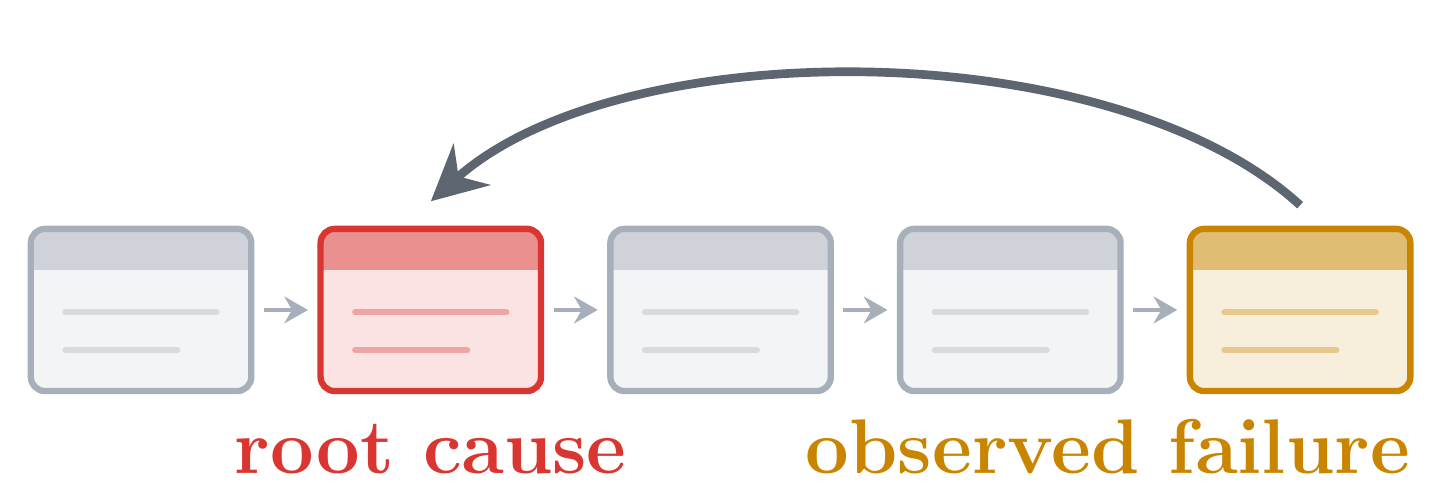
\begin{tikzpicture}[x=1mm,y=1mm, trim left=0mm, trim right=176mm]
      % 5 screens + 4 gaps + the 0.8 mm frame stroke = 176 mm = column width
      \def\sw{28}\def\sh{20.6}\def\sg{8.8}\def\nlast{4}
      \begin{scope}[xshift=0.4mm]
      \foreach \i in {0,...,\nlast}{
        \pgfmathsetmacro{\x}{\i*(\sw+\sg)}
        \ifnum\i=1 \def\c{rootred}\else\ifnum\i=\nlast\relax \def\c{failorange}\else\def\c{basegray}\fi\fi
        \fill[\c!14, rounded corners=1.8mm] (\x,0) rectangle ++(\sw,\sh);
        \fill[\c!55, rounded corners=1.8mm] (\x,\sh-5.2) rectangle ++(\sw,5.2);
        \fill[\c!55] (\x,\sh-5.2) rectangle ++(\sw,2);
        \draw[\c!45, line width=0.8mm, line cap=round] (\x+4.4,10) -- ++(\sw-8.8,0) (\x+4.4,5.2) -- ++(\sw-13.8,0);
        \draw[\c, line width=0.8mm, rounded corners=1.8mm] (\x,0) rectangle ++(\sw,\sh);
        \ifnum\i<\nlast\relax \draw[-{Stealth[length=3mm,width=3.4mm]}, basegray, line width=0.6mm]
          (\x+\sw+1.6,\sh/2) -- ++(\sg-3.2,0);\fi
      }
      \draw[-{Stealth[length=7mm,width=7mm]}, line width=1.1mm, muted]
        ({\nlast*(\sw+\sg)+\sw/2},\sh+3) .. controls ({\nlast*(\sw+\sg)-10},\sh+25) and ({(\sw+\sg)+\sw/2+24},\sh+25)
        .. ({(\sw+\sg)+\sw/2},\sh+3.5);
      \node[anchor=base, text=rootred, font=\small\bfseries, inner sep=0pt] at ({(\sw+\sg)+\sw/2},-10.5) {root cause};
      \node[anchor=base east, text=failorange, font=\small\bfseries, inner sep=0pt]
        at ({\nlast*(\sw+\sg)+\sw},-10.5) {observed failure};
      \end{scope}
    \end{tikzpicture}\par
    \vfill
  \end{minipage}
\end{minipage}\hspace{\gutter}%
\begin{minipage}[t]{\colB}\vspace{0pt}
  \sechead{2}{CUAErrorBench}
  \begin{minipage}[t][\rowAh][t]{\dimexpr\linewidth-\donutD-16mm\relax}\vspace{0pt}
    \raggedright
    \textbf{204 failed OSWorld runs} from 3 agents, each labeled with its root-cause step and error type.\par
    \vfill
    % legend in two columns, in the donut's order (down the first column, then the second)
    {\small\begin{tabular}[t]{@{}l@{\hspace{22mm}}l@{}}
      \legitem{famP}{Perception} & \legitem{famS}{External / System}\\[1.5mm]
      \legitem{famG}{Grounding}  & \legitem{famO}{Others}\\[1.5mm]
      \legitem{famR}{Reasoning}  &
    \end{tabular}\par}
    \vfill
    {\bfseries\color{navy}Reasoning errors dominate; perception and grounding cause 30\%.\par}
  \end{minipage}\hfill
  \begin{minipage}[t]{\donutD}\vspace{0pt}
    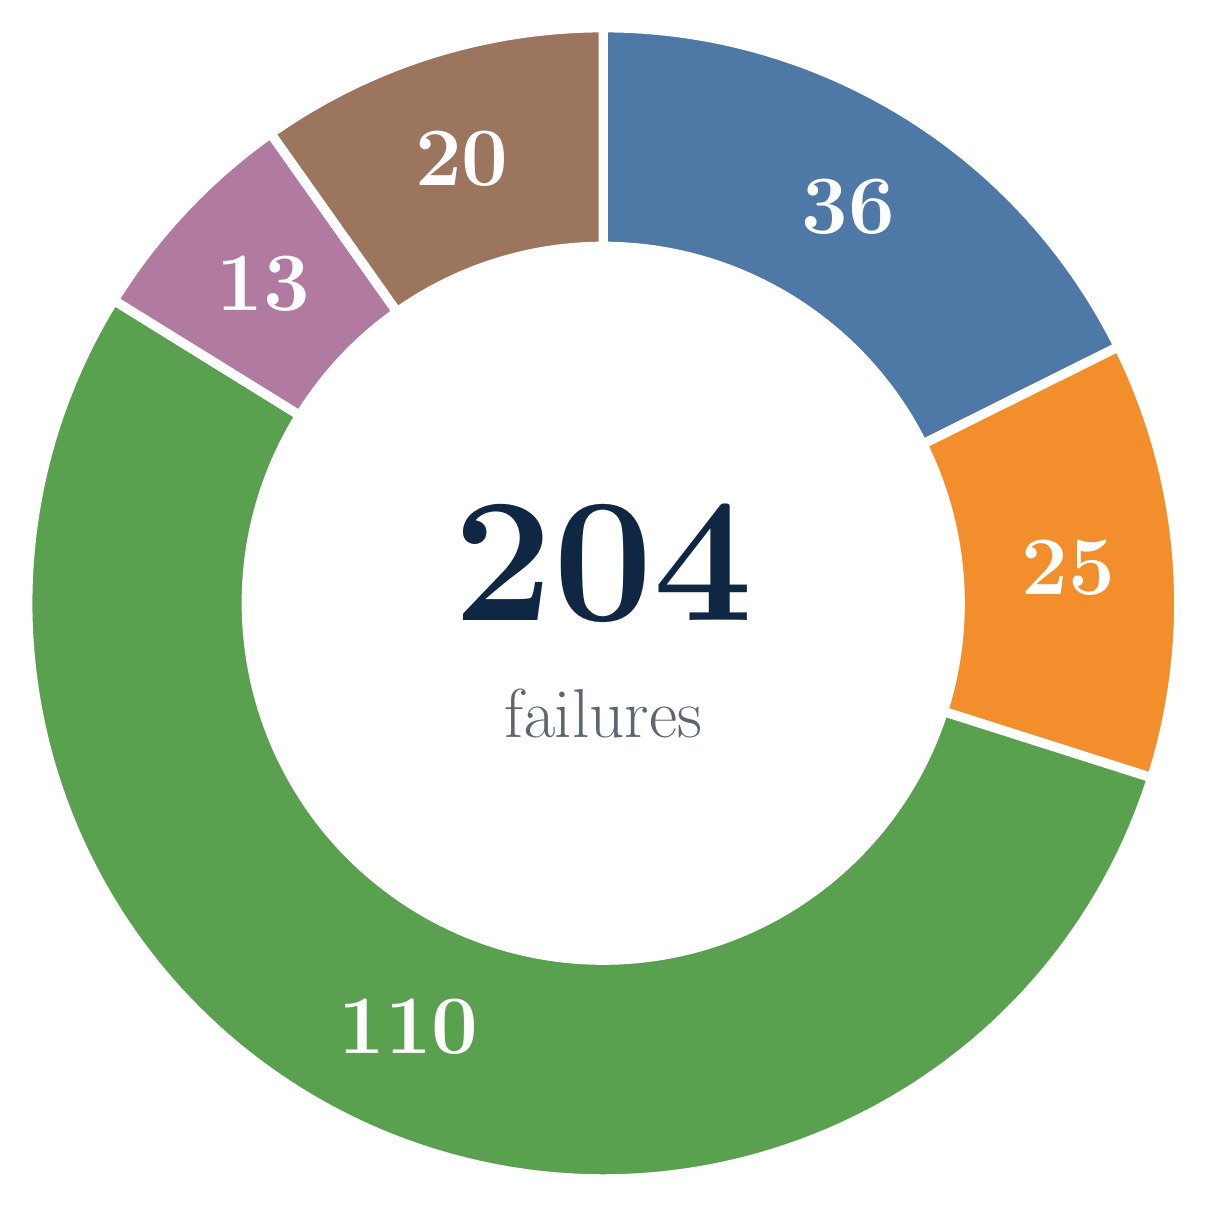
\begin{tikzpicture}[x=1mm,y=1mm]
      \pgfmathsetmacro{\Ro}{0.5*\donutD/1mm}\pgfmathsetmacro{\Ri}{0.62*\Ro}
      \useasboundingbox (-\Ro,-\Ro) rectangle (\Ro,\Ro);
      \foreach \a/\b/\c/\n in {90/26.47/famP/36, 26.47/-17.65/famG/25, -17.65/-211.76/famR/110,
                               -211.76/-234.71/famS/13, -234.71/-270/famO/20}{
        \fill[\c, draw=white, line width=1.2mm] (\a:\Ro) arc[start angle=\a, end angle=\b, radius=\Ro]
          -- (\b:\Ri) arc[start angle=\b, end angle=\a, radius=\Ri] -- cycle;
        \node[font=\fontsize{30pt}{30pt}\selectfont\bfseries, text=white] at ({(\a+\b)/2}:{(\Ro+\Ri)/2}) {\n};
      }
      \node[font=\fontsize{64pt}{64pt}\selectfont\bfseries, text=navy] at (0,5) {204};
      \node[font=\footnotesize, text=muted] at (0,-14) {failures};
    \end{tikzpicture}
  \end{minipage}
\end{minipage}\hspace{\gutter}%
\begin{minipage}[t]{\colC}\vspace{0pt}
  \sechead{3}{Error Taxonomy}
  \begin{minipage}[t][\rowAh][t]{\linewidth}\vspace{0pt}
    \textbf{5 families, 30 subtypes}\par\vfill
    \family{famP}{Perception}{5 subtypes}{Misread what was visible?}\vfill
    \family{famG}{Grounding}{4 subtypes}{Right intent, wrong target?}\vfill
    \family{famR}{Reasoning}{13 subtypes}{Wrong plan chosen or kept?}\vfill
    \family{famS}{External / System}{7 subtypes}{Environment blocked progress?}\vfill
    \family{famO}{Others}{1 subtype}{Infeasible task}
  \end{minipage}
\end{minipage}

\rowsep
% =========================== ROW 2 ===================================
\secheadlede{4}{A Real Failure}{The run fails at \textcolor{failorange}{\textbf{step 12}}, but the mistake
  is made at \textcolor{rootred}{\textbf{step 6}}, where the agent lists \textbf{Kelly} instead of \textbf{Fox}.}
\noindent\teaserfig{\linewidth}\par

\rowsep
% =========================== ROW 3 ===================================
\secheadlede{5}{CUADebugger}{It inspects the before/after screenshots of selected steps, finds the
  earliest error, and writes a report that guides a new run.\par
  For the run above, the re-run \textbf{fails without the report (score~0)} and
  \textcolor{ours}{\textbf{succeeds with it (score~1)}}.}
\noindent\mainfig{\linewidth}\par

\rowsep
% =========================== ROW 4 ===================================
\sechead{6}{Results}
\noindent
\begin{minipage}[t]{\thirdw}\vspace{0pt}
  \paneltitle{Root-cause analysis}{type and step both correct (\%)}
  % \ylabshift: the widest tick labels start flush with the panel title
  \hspace*{-\ylabshift}%
  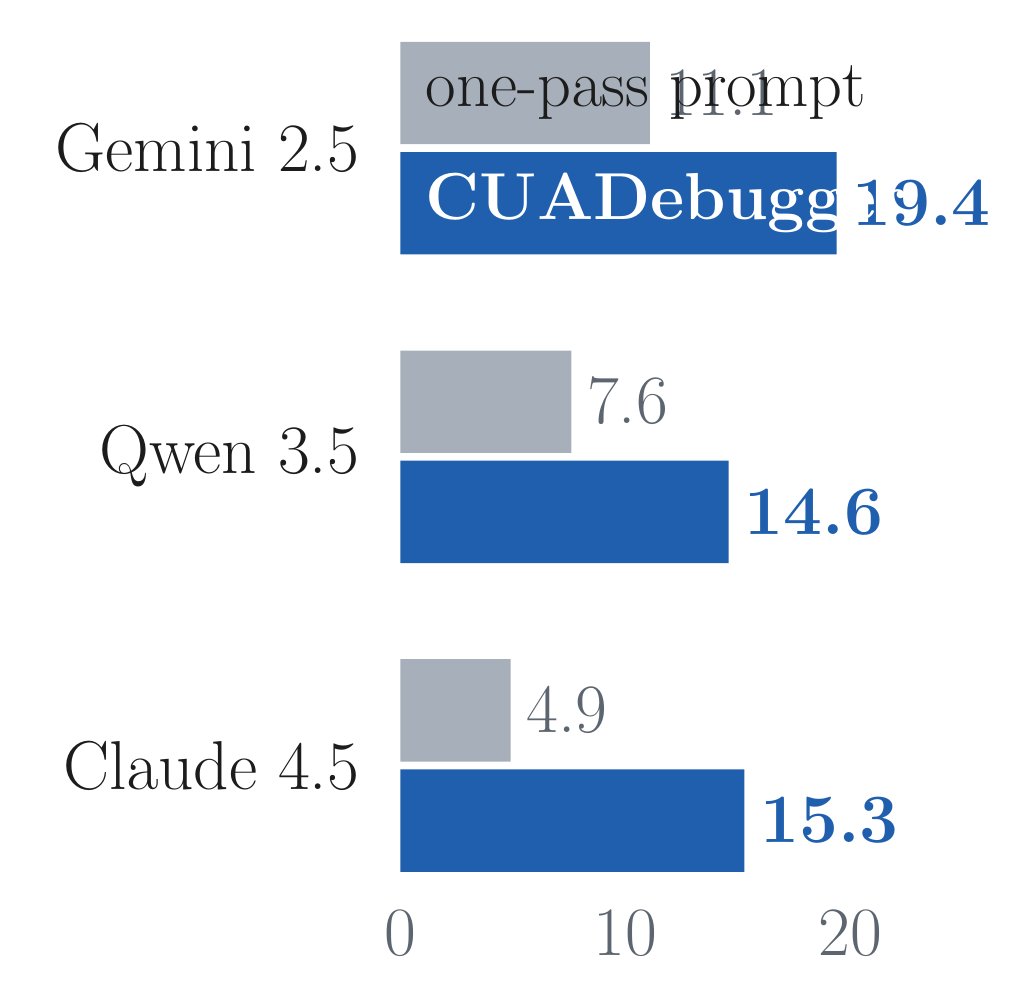
\begin{tikzpicture}
  % ymin/ymax: the outer bars stop 1.8 mm inside the plot area, as in the Recovered chart
  \begin{axis}[hbars, width=\dimexpr\linewidth-68mm+\ylabshift\relax, height=\plotH, bar width=13mm,
      xmin=0, xmax=20, xtick={0,10,20}, ymin=0.6097, ymax=3.3903, ytick={1,2,3},
      yticklabels={Claude 4.5, Qwen 3.5, Gemini 2.5}]
    \addplot[xbar, bar shift=7mm, fill=basegray, draw=none] coordinates {(4.9,1) (7.6,2) (11.1,3)};
    \addplot[xbar, bar shift=-7mm, fill=ours, draw=none] coordinates {(15.3,1) (14.6,2) (19.4,3)};
    \foreach \y/\a/\b in {1/4.9/15.3, 2/7.6/14.6, 3/11.1/19.4}{
      \edef\tmp{\noexpand\node[vlab, text=muted] at ([xshift=0.8mm, yshift=7mm]axis cs:\a,\y) {\a};
                \noexpand\node[vlab, text=ours, font=\noexpand\footnotesize\noexpand\bfseries]
                  at ([xshift=0.8mm, yshift=-7mm]axis cs:\b,\y) {\b};}\tmp}
    % series names written into the top pair of bars (instead of a separate legend)
    \node[anchor=west, font=\fontsize{24pt}{24pt}\selectfont, text=ink, inner sep=0pt]
      at ([xshift=3mm, yshift=7mm]axis cs:0,3) {one-pass prompt};
    \node[anchor=west, font=\fontsize{24pt}{24pt}\selectfont\bfseries, text=white, inner sep=0pt]
      at ([xshift=3mm, yshift=-7mm]axis cs:0,3) {CUADebugger};
  \end{axis}
  \end{tikzpicture}\par
\end{minipage}\hspace{\gutter}%
\begin{minipage}[t]{\thirdw}\vspace{0pt}
  \paneltitle{Re-execution}{accuracy on 361 OSWorld tasks (\%)}
  {\normalsize\arrayrulecolor{rulec}\setlength{\aboverulesep}{0pt}\setlength{\belowrulesep}{0pt}%
   \setlength{\heavyrulewidth}{0.6mm}\setlength{\lightrulewidth}{0.4mm}%
   % six equal rows; with the 2 mm of rules the table is \plotH - 3.6 mm tall and starts
   % 1.8 mm down, so its top and bottom rules line up with the outer bars of the two charts
   % (1.8 mm inside their plot areas); the figures sit centred in their rows
   \def\rs{\rule[-4.5mm]{0pt}{\dimexpr(\plotH-5.6mm)/6\relax}}%
   \setlength{\tabcolsep}{0pt}%
   \vspace*{1.8mm}%
  \begin{tabularx}{\linewidth}{@{}X r@{\hspace{14mm}}r@{}}
    \toprule
    \rs & {\color{muted}Single} & {\color{muted}Continual}\\
    \midrule
    \rs Baseline    & 61.77 & 61.22\\
    \rs Self-debug  & 62.33 & 61.77\\
    \rs Machine RCA & 67.59 & 64.82\\
    \rs\textcolor{ours}{\textbf{CUADebug}} & \textcolor{ours}{\textbf{68.14}} & \textcolor{ours}{\textbf{66.48}}\\
    \midrule
    \rs\textit{Human diagnosis} & \textit{68.98} & \textit{67.87}\\
    \bottomrule
  \end{tabularx}\par}
\end{minipage}\hspace{\gutter}%
\begin{minipage}[t]{\thirdw}\vspace{0pt}
  \paneltitle{\textbf{Recovered failures} {\mdseries(\%)}}{\color{ink}\swatch{basegray}\,\swatch{ours}\ single\quad
    \swatch{basegray!50}\,\swatch{ours!50}\ continual}
  \hspace*{-\ylabshift}%
  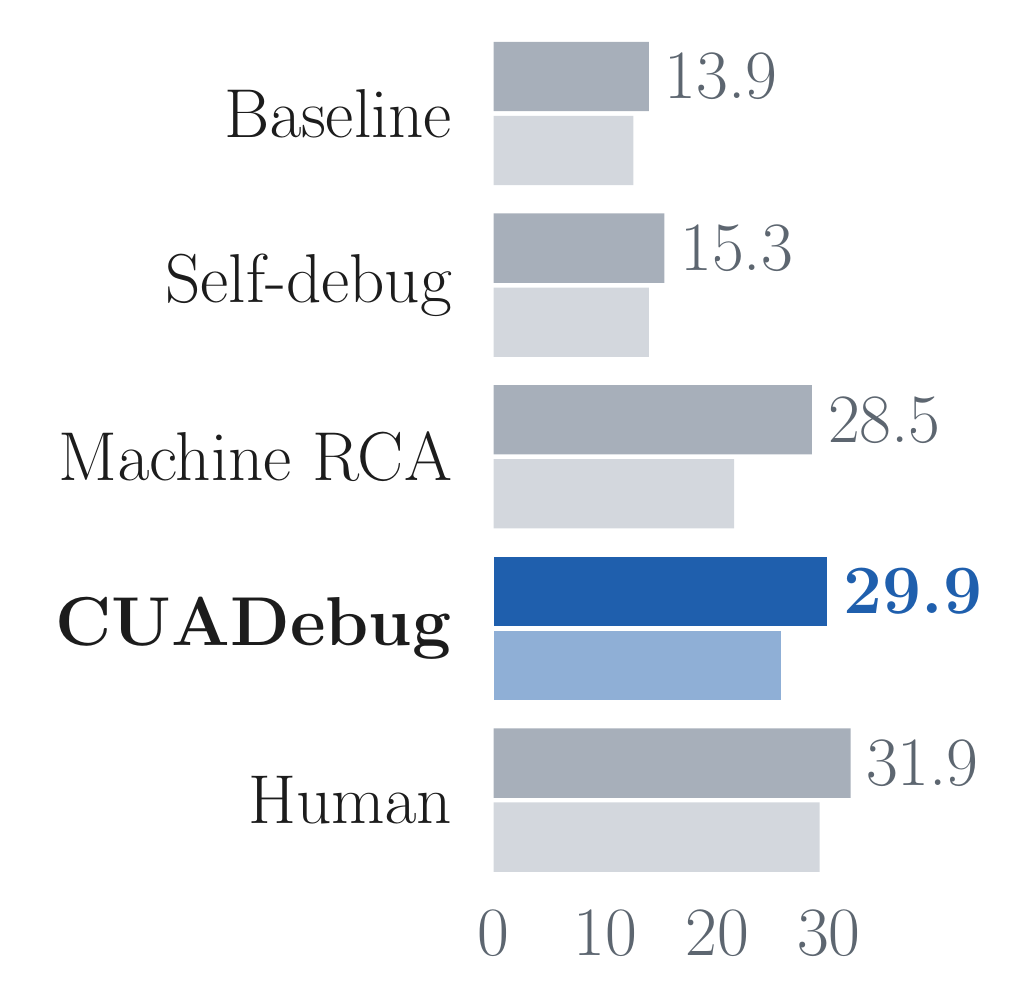
\begin{tikzpicture}
  \begin{axis}[hbars, width=\dimexpr\linewidth-74mm+\ylabshift\relax, height=\plotH, bar width=8.8mm,
      xmin=0, xmax=36, xtick={0,10,20,30}, ymin=0.5, ymax=5.5, ytick={1,2,3,4,5},
      yticklabels={Human, \textbf{CUADebug}, {Machine RCA}, Self-debug, Baseline}]
    \addplot[xbar, bar shift=4.7mm, fill=basegray, draw=none] coordinates {(31.94,1) (28.47,3) (15.28,4) (13.89,5)};
    \addplot[xbar, bar shift=-4.7mm, fill=basegray!50, draw=none] coordinates {(29.17,1) (21.53,3) (13.89,4) (12.50,5)};
    \addplot[xbar, bar shift=4.7mm, fill=ours, draw=none] coordinates {(29.86,2)};
    \addplot[xbar, bar shift=-4.7mm, fill=ours!50, draw=none] coordinates {(25.69,2)};
    % values of the single-run bars, coloured as in the RCA chart (ours bold blue, others muted)
    \foreach \y/\v in {1/31.9, 3/28.5, 4/15.3, 5/13.9}{
      \edef\tmp{\noexpand\node[vlab, text=muted] at ([xshift=0.8mm, yshift=4.7mm]axis cs:\v,\y) {\v};}\tmp}
    \node[vlab, text=ours, font=\footnotesize\bfseries] at ([xshift=0.8mm, yshift=4.7mm]axis cs:29.9,2) {29.9};
  \end{axis}
  \end{tikzpicture}\par
\end{minipage}

\end{document}
